\documentclass[11pt]{article}
\usepackage[T1]{fontenc}
\usepackage{lmodern,amsmath,amssymb,amsthm,booktabs,tikz}
\usepackage[margin=1in]{geometry}
\usepackage[colorlinks=true,linkcolor=blue,citecolor=blue,urlcolor=blue]{hyperref}
\hypersetup{pdfauthor={Qianghao Wu},pdftitle={The configuration LP of restricted assignment need not have a half-integral point at the LP makespan}}
\setlength{\emergencystretch}{3em}
\newtheorem{theorem}{Theorem}
\newtheorem{lemma}[theorem]{Lemma}
\newtheorem{conjecture}{Conjecture}
\theoremstyle{remark}
\newtheorem{remark}[theorem]{Remark}
\newcommand{\cC}{\mathcal{C}}
\newcommand{\cM}{\mathcal{M}}
\newcommand{\CLP}{\mathrm{CLP}}
\newcommand{\LP}{\mathrm{LP}}
\newcommand{\IP}{\mathrm{IP}}
\title{The configuration LP of restricted assignment need not have a half-integral point at the LP makespan}
\author{Qianghao Wu}
\date{November 27, 2026}
\begin{document}
\maketitle
\begin{abstract}
Encz, Mastrolilli and Vercesi conjectured that for every instance $P$ of
the restricted assignment problem, the configuration LP
$\CLP(P,\LP(P))$ at the smallest feasible integer makespan $\LP(P)$
contains a half-integral point (their Conjecture~10). If it were true,
the integrality gap of the configuration LP would reduce to the graph
balancing case. We show that the conjecture is false. Our
counterexample has 12 machines and 20 jobs with processing times 1 and
3, and $\LP(P)=3$. The total processing time is $36=12\cdot 3$, so every
configuration in the support of a feasible point has load exactly 3.
Each such configuration contains 0 or 3 jobs of a fixed set of 4 jobs.
In a half-integral point these 4 jobs are covered 8 times in total, with
weights $1/2$, and 8 is not a multiple of 3. Lean~4 with Mathlib checks
the disproof from the definitions, with only the standard axioms. We
also give a second counterexample with 5 machines and 14 jobs, found by
a random search and checked by an exhaustive search. The
counterexample does not change the known bounds on the integrality gap.

This work has not yet been reviewed by experts. The computations, the
proofs and the text were produced by AI models (from Anthropic and
OpenAI), working under the author's direction.
\end{abstract}
\medskip
\noindent\textbf{Keywords.} Restricted assignment; configuration LP;
half-integrality; integrality gap; scheduling; Lean.

\section{Introduction}
In the restricted assignment problem, $n$ jobs must be assigned to $m$
machines. Job $j$ has a processing time $p_j\in\mathbb{N}_+$ and a set
$\cM_j$ of machines on which it can run. The goal is to minimize the
makespan, the largest total processing time on a machine. In scheduling
notation the problem is $P|\cM_j|C_{\max}$.

The configuration LP is a strong relaxation of this problem. Its
integrality gap is open. Encz, Mastrolilli and Vercesi~\cite{EMV} state
that work on the restricted assignment framework places the gap
$\mathrm{IG}(P|\cM_j|C_{\max})$ between $3/2$ and $11/6$; they cite
Svensson~\cite{Sv}, Jansen and Rohwedder~\cite{JR17}, and Jansen, Land
and Maack (reference~[14] of~\cite{EMV}). For the graph balancing case,
where every job is allowed on at most two machines, they state that the
gap lies between $3/2$ and $1.749$, the upper bound by Jansen and
Rohwedder~\cite{JR18}.

In~\cite{EMV} the authors develop integrality gap preserving reductions
and apply them to several problems, among them the configuration LP of
restricted assignment. In their concluding section they write that the
lack of an understanding of the vertices of this LP prevented a deeper
analysis, and they state the following conjecture, which they
``experimentally asserted for several small-scale instances''
\cite[p.~23:10]{EMV}.

\begin{conjecture}[{\cite[Conjecture~10]{EMV}}]
For every instance $P$ of the restricted assignment problem, the
polyhedron $\CLP(P,\LP(P))$ contains a half-integral feasible solution;
that is, a vector $x$ such that $x_{i,C}\in\{0,\frac12,1\}$ for all
$i\in[m]$ and $C\in\cC_i(P,\LP(P))$.
\end{conjecture}

The authors also report that a stronger version, half-integrality of
every vertex, was disproved by their experiments, and that the version
above had resisted refutation~\cite[p.~23:10]{EMV}. They explain the
motivation: in a half-integral point each job lies in at most two
configurations, so all other machines can be removed from $\cM_j$
without a change of the gap. If the conjecture held, the integrality gap
of the configuration LP of restricted assignment would therefore equal
that of graph balancing, and the bound $1.749$ of~\cite{JR18} would
follow~\cite[p.~23:10]{EMV}.

\begin{theorem}\label{thm:main}
Conjecture~10 of~\cite{EMV} is false. The instance $P^\ast$ of
Section~\ref{sec:instance} has 12 machines, 20 jobs and $\LP(P^\ast)=3$,
and $\CLP(P^\ast,3)$ has no half-integral point.
\end{theorem}

The proof is short (Section~\ref{sec:proof}). It is a parity-type
argument modulo 3. A Lean formalization checks it from the definitions
(Section~\ref{sec:lean}). Section~\ref{sec:second} gives a second, smaller
counterexample that was found by a computer search. The source paper is
from September 2026. We know of no other work that discusses
Conjecture~10.

\section{Definitions}\label{sec:defs}
We use the definitions of~\cite[Section~6]{EMV}. An instance is a matrix
$P=(p_{j,i})$ for jobs $j\in[n]$ and machines $i\in[m]$. In restricted
assignment, $p_{j,i}=p_j\in\mathbb{N}_+$ for $i\in\cM_j$ and
$p_{j,i}=\infty$ otherwise. For an integer $T$, the configurations of
machine $i$ are
\begin{equation}\label{eq:conf}
\cC_i(P,T)=\Bigl\{C\subseteq[n] : \sum_{j\in C}p_{j,i}\le T\Bigr\}.
\end{equation}
A configuration is a set of jobs, so it contains each job at most once.
Its load is at most $T$, not necessarily equal to $T$. A configuration
of machine $i$ that contains a job $j$ with $i\notin\cM_j$ has infinite
load, so every configuration of $i$ consists of jobs allowed on $i$.
We write $p(C)=\sum_{j\in C}p_j$. The polyhedron $\CLP(P,T)$ is the set of
vectors $x=(x_{i,C})_{i\in[m],\,C\in\cC_i(P,T)}$ with
\begin{align}
\sum_{C\in\cC_i(P,T)}x_{i,C}&=1, && i\in[m],\label{eq:mach}\\
\sum_{i\in[m]}\ \sum_{C\in\cC_i(P,T):\,j\in C}x_{i,C}&=1, && j\in[n],\label{eq:job}\\
x_{i,C}&\ge 0, && i\in[m],\ C\in\cC_i(P,T).\label{eq:nonneg}
\end{align}
$\LP(P)$ is the smallest integer $T$ for which $\CLP(P,T)$ is
feasible~\cite[p.~23:8]{EMV}. A point is half-integral if all its
entries lie in $\{0,\frac12,1\}$.

The following identity is standard. For a point $x\in\CLP(P,T)$ and
weights $w\colon[n]\to\mathbb{R}$, write $w(C)=\sum_{j\in C}w_j$. Then
\begin{equation}\label{eq:count}
\sum_{i\in[m]}\sum_{C\in\cC_i(P,T)}x_{i,C}\,w(C)=\sum_{j\in[n]}w_j .
\end{equation}
To prove it, exchange the sums and apply~\eqref{eq:job}. With $w=p$,
\eqref{eq:mach}, \eqref{eq:nonneg} and $p(C)\le T$ give the volume bound
\begin{equation}\label{eq:volume}
\sum_{j\in[n]}p_j=\sum_{i}\sum_{C}x_{i,C}\,p(C)\le\sum_i\sum_C x_{i,C}\,T=mT .
\end{equation}

\section{The counterexample}\label{sec:instance}
The machines are the pairs $(c,t)$ with a \emph{copy} $c\in\{0,1,2\}$
and $t\in\{0,1,2,3\}$, so $m=12$. There are two kinds of jobs, so $n=20$.
\begin{itemize}
\item \emph{Point jobs} $P(c,k)$ for $c\in\{0,1,2\}$, $k\in\{0,1,2,3\}$:
size 1, allowed on the three machines $(c,t)$ with $t\neq k$.
\item \emph{Filler jobs} $F(f)$ for $f\in\{0,\dots,7\}$: size 3. Machine
$(c,t)$ allows $F(2t)$ and $F(2t+1)$. So $F(f)$ is allowed on the three
machines $(0,\lfloor f/2\rfloor)$, $(1,\lfloor f/2\rfloor)$,
$(2,\lfloor f/2\rfloor)$.
\end{itemize}
Each machine allows exactly 5 jobs: 3 point jobs of its own copy and 2
fillers. Within one copy, the 4 machines correspond to the 4 subsets of
size 3 of the 4 point jobs (Figure~\ref{fig:copy}). The total
processing time is $12\cdot 1+8\cdot 3=36$.

\begin{figure}[ht]
\centering
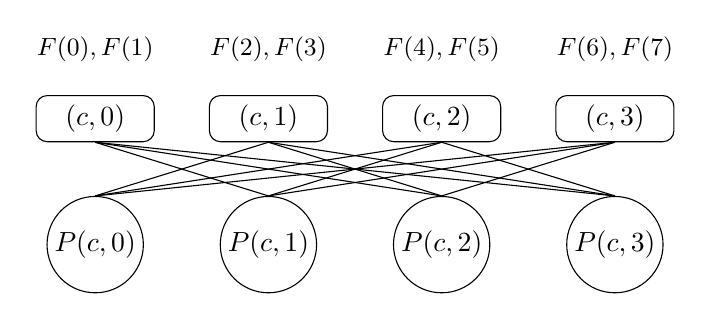
\begin{tikzpicture}[x=2.2cm,y=1.6cm]
\foreach \t in {0,1,2,3} {
  \node[draw,rounded corners,minimum width=1.5cm] (m\t) at (\t,1) {$(c,\t)$};
  \node[draw,circle,inner sep=1.5pt] (p\t) at (\t,0) {$P(c,\t)$};
}
\foreach \t in {0,1,2,3} { \foreach \k in {0,1,2,3} {
  \ifnum\t=\k\else \draw (m\t.south) -- (p\k.north); \fi
}}
\foreach \t in {0,1,2,3} {
  \node[font=\small] at (\t,1.55) {$F(\the\numexpr2*\t\relax),F(\the\numexpr2*\t+1\relax)$};
}
\end{tikzpicture}
\caption{One copy $c$ of the instance. A line joins a machine and a
point job that it allows. Above each machine are its two filler jobs;
these are shared by the machines $(0,t)$, $(1,t)$, $(2,t)$.}
\label{fig:copy}
\end{figure}

\subsection{The proof}\label{sec:proof}

\begin{lemma}\label{lem:lp}
$\LP(P^\ast)=3$.
\end{lemma}
\begin{proof}
If $T\le 2$, the volume bound~\eqref{eq:volume} would give
$36\le 12T\le 24$, so $\CLP(P^\ast,T)$ is empty. For $T=3$, let $x$ have
the value $\frac13$ on every configuration of load exactly 3, and $0$
on all other configurations. A configuration of load exactly 3 on
machine $(c,t)$ is either a single filler, or the set of its three
point jobs, because a filler and a point job together have load 4. So
each machine has exactly 3 such configurations, and~\eqref{eq:mach}
holds. Each filler lies in such a configuration on each of its 3
machines. Each point job $P(c,k)$ lies in the three-point configuration
of each of its 3 machines. So~\eqref{eq:job} holds, and $x$ is a point
of $\CLP(P^\ast,3)$.
\end{proof}

Within one copy, this point puts weight $\frac13$ on each of the 4
subsets of size 3 of a 4-set. These are the only full configurations
that contain point jobs, and the fillers fill the remaining capacity.

\begin{lemma}\label{lem:full}
If $x\in\CLP(P^\ast,3)$ and $x_{i,C}>0$, then $p(C)=3$.
\end{lemma}
\begin{proof}
The total processing time is $36=12\cdot 3=mT$. So~\eqref{eq:volume}
holds with equality, that is,
$\sum_i\sum_C x_{i,C}\,(3-p(C))=0$. Each term is nonnegative, so each
term is zero.
\end{proof}

Lemma~\ref{lem:full} is where configurations of load less than 3 are
excluded. Such configurations exist (for example a single point job),
and they can contain 1 or 2 point jobs of copy 0. The tight volume
shows that they get weight 0 in every feasible point.

\begin{proof}[Proof of Theorem~\ref{thm:main}]
Let $w_j=1$ if $j$ is a point job $P(0,k)$ of copy 0, and $w_j=0$
otherwise; so $\sum_j w_j=4$. Every configuration $C$ with $p(C)=3$
satisfies $w(C)\in\{0,3\}$: a single filler has $w(C)=0$, and the
three point jobs of machine $(c,t)$ have $w(C)=3$ if $c=0$ and $0$
otherwise. Suppose that $x\in\CLP(P^\ast,3)$ is half-integral, and let
$y=2x$. Then $y$ is a vector of nonnegative integers. By~\eqref{eq:count}
with the weights $w$,
\[
\sum_i\sum_C y_{i,C}\,w(C)=2\sum_j w_j=8 .
\]
By Lemma~\ref{lem:full}, every term with $y_{i,C}\neq0$ has $p(C)=3$,
so $w(C)\in\{0,3\}$. So the left side is a multiple of 3. But 8 is not
a multiple of 3. So $\CLP(P^\ast,3)=\CLP(P^\ast,\LP(P^\ast))$ has no
half-integral point.
\end{proof}

\begin{remark}
The same argument excludes every point of $\CLP(P^\ast,3)$ whose
entries are rationals with denominators prime to 3: if $d$ is such a
common denominator, then $\sum y\,w=4d$ for $y=dx$, and $3\nmid 4d$.
In particular $\CLP(P^\ast,3)$ has no integral point. An explicit
assignment with makespan 4 exists: machines $(0,t)$ and $(1,t)$ take
$F(2t)$ and $F(2t+1)$ respectively, and each machine $(c,t)$ takes
$P(c,t+1\bmod 4)$. So $\IP(P^\ast)=4$, and the integrality gap of
$P^\ast$ is $4/3$. This is less than $3/2$, so $P^\ast$ does not
improve the known lower bound on the integrality gap.
\end{remark}

The construction uses three copies for a reason of volume. In the point of Lemma~\ref{lem:lp},
the triples carry weight $\frac13$ on each of the 4 machines, and the
other $\frac23$ of each machine must be filled by fillers of size 3.
Each filler needs total weight 1, so the number of fillers is
$\frac23\cdot 4c$ for $c$ copies. This is an integer for $c=3$, which
gives the 8 fillers.

\section{A second counterexample}\label{sec:second}
A random walk among small instances with an integrality gap found a
second counterexample. It has 5 machines (indexed from 0), 14 jobs
and $\LP(P)=14$. For the jobs $j=0,\dots,13$, the processing times are
\[
(p_0,\dots,p_{13})=(1,5,1,5,1,6,1,10,8,3,4,9,6,8),
\]
and the sets $\cM_0,\dots,\cM_{13}$ are
\[
\begin{gathered}
\{1,4\},\ \{1,2,4\},\ \{2,3\},\ \{1,4\},\ \{2,3,4\},\ \{1,2,3,4\},\ \{0,1,3\},\\
\{3,4\},\ \{0,1,2,3\},\ \{2\},\ \{2,4\},\ \{0,1,2\},\ \{0,1,2,3,4\},\ \{1\}.
\end{gathered}
\]
The total processing time is $68>5\cdot 13=65$, so $\CLP(P,13)$ is
empty by~\eqref{eq:volume}. The file \texttt{instance\_small.json} in the folder \texttt{checks/}
gives a point of $\CLP(P,14)$ with 12 nonzero entries, all equal to
$\frac13$ or $\frac23$. The machines have 9, 74, 105, 49 and 70
configurations at $T=14$. An exhaustive search shows that
$\CLP(P,14)$ has no half-integral point. We have no short proof for
this instance, and it is not checked in Lean. The volume here is not
tight ($68<70$), so the argument of Section~\ref{sec:proof} does not
apply directly.

\section{How the result was checked}\label{sec:check}

\subsection{Lean}\label{sec:lean}
The file \texttt{lean/Solution.lean} states the definitions of
Section~\ref{sec:defs} in Lean~4 with Mathlib (both at v4.36.0) and
proves the theorem \texttt{HalfIntegralCLP.not\_conjecture10}, whose statement is $\neg$\,\texttt{Conjecture10}.
The definitions are as follows.
\begin{itemize}
\item An instance has $n$ jobs \texttt{Fin n} and $m$ machines
\texttt{Fin m}, a size function $p\colon$\texttt{Fin n}$\to\mathbb{N}$
with $p_j>0$, and sets $\cM_j$.
\item The configurations $\cC_i(P,T)$, for an integer $T$, are the subsets
of the jobs allowed on $i$ whose load is at most $T$. This is the
reading of~\eqref{eq:conf} with $p_{j,i}=\infty$ for $i\notin\cM_j$.
\item A point is a real function $x_{i,C}$. The constraints
\eqref{eq:mach}--\eqref{eq:nonneg} refer only to the entries with
$C\in\cC_i(P,T)$.
\item \texttt{Conjecture10} says: for all $n$, $m$, all instances $P$
and all integers $T$, if $T$ is the least element of
$\{T\in\mathbb{Z}:\CLP(P,T)\neq\emptyset\}$, then $\CLP(P,T)$ has a
point with every entry $x_{i,C}$, $C\in\cC_i(P,T)$, in
$\{0,\frac12,1\}$.
\end{itemize}
The proof follows Section~\ref{sec:proof}: identity~\eqref{eq:count} and
the volume bound are proved for all instances. The finite facts about
$P^\ast$ (the total size 36, the 3 full configurations of each machine,
the coverage of each job, and $w(C)\in\{0,3\}$ for each full
configuration) are proved by evaluation in the Lean kernel
(\texttt{decide +kernel}). The command \texttt{\#print axioms} reports
only \texttt{propext}, \texttt{Classical.choice} and \texttt{Quot.sound}.
The file compiles in about 18~s on one core after Mathlib is built.
The file \texttt{lean/Challenge.lean} repeats the definitions and the
statement with \texttt{sorry}, and \texttt{lake comparator} confirms that
the proof proves exactly this statement.

\subsection{Python}
The folder \texttt{checks/} has exact checks that use only the Python
standard library (integers and \texttt{fractions.Fraction}).
\begin{itemize}
\item \texttt{check\_certificate.py} checks the point of
Lemma~\ref{lem:lp}, the volume facts, and $w(C)\equiv 0\pmod 3$ for all
36 configurations of load 3 (3 on each of the 12 machines).
\item \texttt{vcheck.py} is a second checker, written separately from the
first. It enumerates $\cC_i(P,T)$ from~\eqref{eq:conf} (10
configurations per machine for $P^\ast$ at $T=3$), decides the
feasibility of $\CLP(P,T)$ and $\CLP(P,T-1)$ with an exact rational
simplex method, and decides whether a half-integral point exists with an
exhaustive search. The search does not use the argument modulo 3. For
$P^\ast$ it visits 2227 nodes and finds no point; as a control, it finds
a half-integral point at $T=4$. For the second instance it visits
155269 nodes and finds no point.
\item \texttt{control.py} compares the pruned search of
\texttt{vcheck.py} with a search without pruning on 400 random small
instances for each of the seeds 1 and 2. All answers agree (282 and 281
of the instances have a half-integral point).
\item \texttt{check\_small.py} checks the second counterexample again,
with the point check and the search of \texttt{check\_counterexample.py},
which share no code with \texttt{vcheck.py}.
\item \texttt{check\_ip.py} checks the assignment with makespan 4.
\end{itemize}

\section{Limits}
\begin{itemize}
\item The result disproves Conjecture~10 as stated. It does not change
the known bounds on the integrality gap of the configuration LP for
restricted assignment. The instance $P^\ast$ has gap $4/3$.
\item The result closes the route of~\cite[p.~23:10]{EMV} from
half-integral points to graph balancing. It does not show that the gap
of restricted assignment differs from that of graph balancing.
\item We did not study weaker forms of the conjecture or other routes
from restricted assignment to graph balancing.
\item Conjecture~10 appeared in September 2026. We found no other work
that discusses it. Its importance comes from the reduction that its
authors describe.
\item The second counterexample relies on an exhaustive computer search.
Only the first counterexample is checked in Lean.
\end{itemize}

\begin{thebibliography}{9}
\bibitem{EMV}
K.~I. Encz, M.~Mastrolilli and E.~Vercesi,
\emph{Integrality gap preserving reductions},
preprint, September 17, 2026,
\href{https://arxiv.org/abs/2609.19967v1}{arXiv:2609.19967v1}.
Conjecture~10 is on page 23:10; the definitions are on page 23:8.
\bibitem{JR17}
K.~Jansen and L.~Rohwedder,
\emph{On the configuration-LP of the restricted assignment problem},
Proceedings of the Twenty-Eighth Annual ACM-SIAM Symposium on Discrete
Algorithms (SODA 2017), 2670--2678.
Preprint \href{https://arxiv.org/abs/1611.01934}{arXiv:1611.01934}.
\bibitem{JR18}
K.~Jansen and L.~Rohwedder,
\emph{Local search breaks 1.75 for graph balancing},
preprint, November 2, 2018,
\href{https://arxiv.org/abs/1811.00955}{arXiv:1811.00955}.
\bibitem{Sv}
O.~Svensson,
\emph{Santa Claus schedules jobs on unrelated machines},
Proceedings of the 43rd Annual ACM Symposium on Theory of Computing
(STOC 2011), 617--626.
\href{https://doi.org/10.1145/1993636.1993718}{doi:10.1145/1993636.1993718}.
\end{thebibliography}
\end{document}
